\begin{figure}[h]
    \centering
    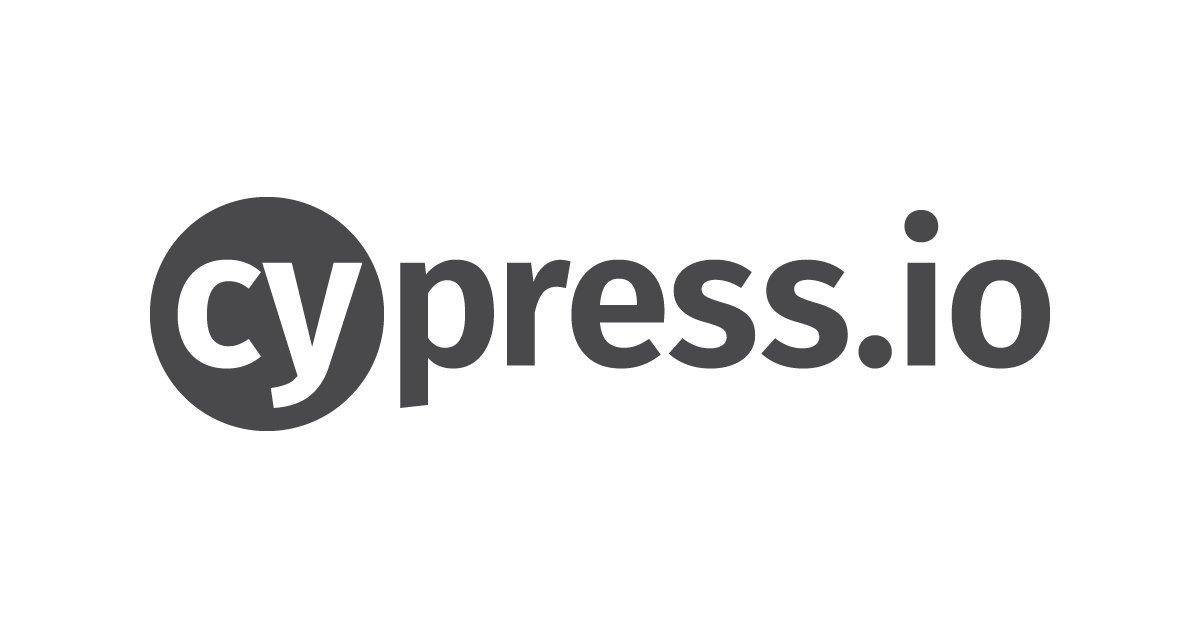
\includegraphics[width=0.5\linewidth]{pics/cypress-logo.png}
    \caption{Cypress}
    \label{fig:enter-label}
\end{figure}


Cypress is ein sehr neuer Testrunner, welcher JavaScript Tests automatisch ausführen kann.
Cypress unterstützt drei verschiedene Arten von Tests:

\begin{itemize}
\item \textbf{End-to-End-Tests}
\item \textbf{Integration-Tests}
\item \textbf{Unit-Tests}
\end{itemize}

In dieser Diplomarbeit wurde Cypress benutzt um Frontend aber sowohl auch API-Tests zu schreiben
\cite{Cypress}
\subsection{API Test}
Mit einem API (Application Programming Interface) Test kann festgestellt werden ob die Anforderungen in Sachen Funktionalität, Leistung, Zuverlässigkeit und Sicherheit erfüllen. Das Ziel eines solchen Test ist es Fehler oder unerwartete Verhaltenswiesen zu finden. So stellt man sicher, dass der Endbenutzer kein fehlerhaftes oder unsichers Produkt zur Verfügung gestellt bekommt. 

Dennoch gestalten sich API-Tests oft komplexer als gedacht. APIs bedienen sich in der Regel Protokollen und Standards, mit denen Sie normalerweise nicht direkt interagieren. Diese Normen sind unerlässlich, um die Kommunikation zwischen verschiedenen Plattformen, Anwendungen und Systemen zu ermöglichen. Daher ist es erforderlich, nicht nur die Funktionalität einer API zu prüfen, sondern auch ihre Leistung, Sicherheit und das reibungslose Zusammenspiel aller Komponenten, um eine zuverlässige Schnittstelle zu gewährleisten.

\subsubsection{Welche verschiedenen Arten von API Tests gibt es?}

Die Art der Tests hängt davon ab was genau zu testen ist. Es gibt eine Vielzahl von verschiedene Arten von Tests:

\begin{itemize}
    \item \textbf{Funktionstests}
        \newline
        Mit dieser Art von Tests werden verschiedene Funktion der API getestet.
    \item \textbf{Zuverlässigkeitstests}
        \newline
        Hier wird überprüft, ob die API innerhalb von einer bestimmten Zeitspanne ohne Ausfälle funktioniert.
    \item \textbf{Lasttest}
        \newline
        Hierbei wird die Leistung der API überprüft. 
    \item \textbf{Sicherheitstest}
        \newline
        Bei diesen Tests wird sichergestellt, das keine externen Personen Zugriff auf geschützte Daten bekommen.
    \item \textbf{Endpunkt-Tests}
        \newline
        Hierbei wird überprüft, ob die API korrekt entwickelt wurde und ob jeder Enpunkt problemlos funktioniert.
\end{itemize}

\subsubsection{Beispiel eines API Tests}
\begin{lstlisting}
it('get all projects', () => {
        cy
            .request({
                method: 'POST',
                url: 'http://localhost:3000/api/v1/login',
                failOnStatusCode: false,
                body: {
                    email: 'write@domain.com',
                    password: Cypress.env('password')
                }
            }).then((xhr) => {
                cy
                    .request({
                        method: 'GET',
                        url: 'http://localhost:3000/api/v1/projects',
                        failOnStatusCode: false,
                        headers: {
                            authorization: `Bearer ${xhr.body.data.auth_token}`
                        }
                    }).then((xhr) => {
                        expect(xhr.body.data.projects.length).to.eq(7)
                    })
            })
    })
\end{lstlisting}

Jeder Cypress Test beginnt immer mit "it('<name>', () => {})" in der Arrow Function start dann der Test. Dieser beginnt immer mit "cy". Alles was danach kommt hat immer einen Punkt vor sich, in diesem Fall will man einen Request testen, daher nennt sich diese Funktion ".request({})" Als Übergabeparameter braucht es dann hier die Methode welche verwendet werden soll also entweder POST, PUT, GET oder DELETE. Weiters wird eine URL benötigt auf welche der Request abzielen soll. Nun kann noch ein Body Objekt und eine failOnStatusCode Flag hinzugefügt werden. Wird diese auf true gesetzt failed der Test sobald ein Request einen StatusCode im 400er Bereich zurückbekommt. Diese Option gibt es daher, weil es auch vorkommen kann, das man testen will wie das Programm im Error-Fall reagiert.
\cite{API_Tests}
\subsection{APP Test}
Mit einem wie oben beschriebenen API Test wird das Backend getestet. Mit einem APP Test hingegen wird das Frontend auf Fehler überprüft. Hierbei wird die Anwendung auf Funktionstüchtigkeit, Leistung, Nutzerfreundlichkeit und Sicherheit getestet

Zu den verschiedenen Kategorien der APP-Tests gehören:

\begin{itemize}
    \item \textbf{Funktionstests}
        \newline
        Der Funktionstest gewährleistet die ordnungsgemäße Funktionsweise der App gemäß den vorgegebenen Zielen. Typischerweise sind diese Ziele bereits festgelegt. Dabei müssen Standard-Softwareoperationen wie Installation, Deinstallation, sämtliche In-App-Funktionen sowie das Minimieren und Wiederaufrufen der App fehlerfrei durchgeführt werden.
    \item \textbf{Usability-Tests}
        \newline
        Für diesen Usability-Test werden Probanden herangezogen, um die Benutzerfreundlichkeit Ihrer Anwendung und ihr Layout zu bewerten. Idealerweise sollten die Probanden Ihrer geplanten Zielgruppe angehören, um aussagekräftigere Ergebnisse zu erzielen. Die potenziellen Nutzer erkunden Ihre App und prüfen, wie reibungslos die Navigation funktioniert, wie einfach der Zugriff auf wichtige Funktionen ist und ob Icons, Links und Texte gut erreichbar und ausreichend groß sind.
    \item \textbf{Penetrationstests}
        \newline
        Bei der Entwicklung mobiler Apps sollte ein Schwerpunkt auf Sicherheit gelegt werden, insbesondere auf den Schutz der Nutzerdaten. Penetrationstests bieten eine effektive Methode, um Sicherheitsschwachstellen aufzudecken. Ein erfahrenes Testteam sollte versuchen, in das System einzudringen und potenzielle Sicherheitsprobleme zu identifizieren. Auf diese Weise können potenzielle Datenlecks frühzeitig erkannt und Maßnahmen ergriffen werden, um einen Diebstahl von Daten zu verhindern.
\end{itemize}



\subsection{Integration von Cypress}
Die Installation von Cypress erfolgt meist über einen Paketmanager, hierbei kann entweder npm oder yarn verwendet werden. Ansonsten kann Cypress besteht auch noch die Möglichkeit Cypress direkt über die offiziele Website herunterzuladen (https://docs.cypress.io/guides/getting-started/installing-cypress).
Im Projektverzeichnis muss der Befehl:

\begin{lstlisting}
    npm install cypress --save-dev -> Fuer NPM
    yarn add cypress --dev -> Fuer Yarn
\end{lstlisting}

ausgeführt werden.
Nun sollte sich der Ordner "cypress" im Projektverzeichnis befinden. Dieser enthält mehrere Unterordner, welche jedoch nicht weiter relevant sind. Wenn alles installiert ist kann Cypress über den Befehl:

\begin{lstlisting}
    npx cypress open -> Fuer NPM
    yarn run cypress open -> Fuer Yarn
\end{lstlisting}

ausgeführt werden.
\cite{Integration_von_Cypress}

\subsubsection{Erstellung eines simplen Testfalls}
Im folgenden Testbeispiel wird überprüft ob die Projektsuchen funktioniert. Im ersten Schritt wird in die Suchleiste der Titel eingegeben. Danach wird anhand von den angezeigten Eigenschaften des Projekts überprüft, ob auch das richtige Projekt vom Such-Algorithmus gefunden wurde. 

\begin{lstlisting}
describe('Project template spec', () => {
    beforeEach(() => {
        cy
            .FIXTURES_setupBasicProjects()

})
    
    it('search for projects - title ', () => {
        cy
            .authenticateAs("test@domain.com")
            .visit('projects')
            .getId('email-search')
            .type('1 Fixture-Project')
            .get('[data-testid="email-search"] [data-testid="submit-search"]')
            .click()
            .getId('project-title-0')
            .should('contain', 'Fixture-Project')
            .getId('project-created-0')
            .should('contain', '28.04.2017 02:17')
            .getId('project-storage-0')
            .should('contain', '5.74 MB')
    })
\end{lstlisting}

Der Test beginnt mit einem "describe()" in diesem Block befindet sich eine kurze Zusammenfassung und der "beforeEach()" Block. Dieser wird vor jedem Test neu ausgeführt und lädt in diesem Fall die Testdaten aus den Fixtures.

Der eigentliche Test beginnt dann beim "it()" Block. Als erstes Authentifiziert sich der User und besucht die Seite "projects". Danach sucht der nach der data-testid "email-search" wählt diese aus und schreibt in diese den Projekt Titel nach welchem gesucht werden soll. In weiterer Folge wird danach der Submit Button gedrückt und wieder mit einer data-testid nach den Eigenschaften des gefundenen Projekts geschaut.

\subsubsection{Ausführung des Testfalls}

Um den Testfall danach auszuführen muss der Testrunner zunächst mit dem Befehl:

\begin{lstlisting}
    npx cypress open -> Fuer NPM
    yarn run cypress open -> Fuer Yarn
\end{lstlisting}

gestartet werden.
Im Anschluss kann muss der richtige Test ausgewählt werden und es öffnet sich ein neues Fenster in dem der Test ausgeführt wird. Auf der rechten Seite des neuen Fensters befindet sich ein Vorschau Fenster durch welches man immer den aktuellen Status des Tests beobachten kann und auf der linken Seite wird genau dokumentiert welcher Schritt gerade ausgeführt wird.

\subsection{Vor und Nachteile von Cypress}

Die Intention der Entwickler von Cypress war es, das Testen im Browser zu vereinfache. Das Einbinden von Cypress in eine Applikation ist sehr einfach, es braucht keine extra Konfiguration. Auch das Verständnis der Sytnax ist sehr einfach. Ein großer Pluspunkt in Cypress ist, dass das warten auf DOM-Elemente mithilfe eines Mechanismus vereinfacht wurde. Funktionen wie "sleep" oder "wait" entfallen also. 
Zwei Nachteile die Cypress besitzt sind, dass es JavaScript Kenntnisse voraussgesetzt sind. Selenium hingegen unterstützt mehrere Sprachen. Außerdem wird nur Chrome als auführender Browser unterstützt.












